% This is the tex file for ISVLSI16 submission
% by Kaiyuan Guo

%\documentclass{sig-alternate-05-2015}
  \documentclass[10pt, conference]{IEEEtran}
    
    \usepackage{amsmath,amsfonts,amssymb}
    \usepackage{graphicx}
    \usepackage{subfigure}
    %\usepackage{algpseudocode}
    %\usepackage{algorithm}
    \usepackage{caption}
    \usepackage{multirow}
    \usepackage{textcomp,booktabs}
    \usepackage[usenames,dvipsnames]{color}
    \usepackage{colortbl}
    \usepackage{indentfirst}
    \usepackage{url}
    \usepackage{cite}
    \usepackage{bibspacing}
    \usepackage{threeparttable}
    \usepackage{bigstrut}
    \usepackage{clrscode3e}
    
    \newcommand{\PreserveBackslash}[1]{\let\temp=\\#1\let\\=\temp}
    \newcolumntype{C}[1]{>{\PreserveBackslash\centering}p{#1}}
    \newcolumntype{R}[1]{>{\PreserveBackslash\raggedleft}p{#1}}
    \newcolumntype{L}[1]{>{\PreserveBackslash\raggedright}p{#1}}
    
    \begin{document}
    
    % title
    \title{\Large\textbf{RRAM Based Buffer Design for Energy Efficient CNN Accelerator}}
    
    \author{
       %   Kaiyuan Guo
       %   Yiming Hu
       %   Jincheng Yu
       %   Xuefei Ning
       %   Yu Wang
       %   Huazhong Yang
    }
    
    \maketitle
    
    \begin{abstract}
    
Convolutional Neural Network (CNN) has become the state-of-the-art algorithm for many computer vision tasks. But its high computation complexity and high memory complexity makes it hard to be applied with traditional platforms like CPUs. Memory energy can take up more than 50\% of the system energy, which limits the energy efficiency of CNN processing. The emerging metal-oxide resistive switching random-access memory (RRAM) has been widely studied because of its good properties like high storage density and the compatibility with CMOS. In this paper, a system level energy analysis of using RRAM as on-chip weight buffer is carried out for a typical CNN accelerator. Hardware and scheduling optimizations are proposed to fully utilize the large RAM and avoid high read/write energy overhead. Experimental results show that RRAM based design saves $12-18\%$ system energy with a $15-75\%$ smaller on-chip RAM area compared with SRAM design.
    
\end{abstract}    
    
    \section{Introduction}

Convolutional Neural Network (CNN) has become a state-of-the-art algorithm for a wide range of applications like image classification~\cite{simonyan2014very}\cite{he2015deep} , object detection~\cite{redmon2015you} and other image based tasks. Compared with traditional hand-crafted feature based methods, CNN introduces a uniform model for different tasks and adjusts the model based on different training data set. Thus CNN can be adopted in different tasks and keeps high classification accuracy or detection accuracy.

But CNN is still not widely applied in real applications because of its high computation and memory complexity. A typical network like AlexNet~\cite{krizhevsky2012imagenet} consists of more than 240MB parameters and 1.4GFLOPs for the inference of a single $224\times 224$ image. More advanced networks~\cite{simonyan2014very}\cite{he2015deep} requires much more computation and memory than AlexNet. The energy cost for CNN computation is thus high, especially on traditional platforms like CPU.

Various works explore energy efficient hardware designs for CNN accelerators. One kind of researches base on CMOS technology and focus on efficient data path and memory system designs, for example the data tiling strategy in~\cite{zhang2015optimizing} and the convolution kernel in~\cite{qiu2016going}\cite{du2015shidiannao}. In these designs, the on-chip memory is implemented with SRAM, which means the size is quite limited. Thus external memory like DRAM is always needed in real applications, which means a large energy cost on the off-chip data transfer. This energy cost greatly limits the energy efficiency of this kind of design.

One solution to reduce memory access is to perform in memory computing. RRAM cross bar based design is one of the popular research topics. Chi, et al. proposes the PRIME~\cite{chi2016prime} architecture which implements the matrix vector multiplication directly with the RRAM cross bar. Work by Cheng et al.~\cite{cheng2017time} implements the RRAM cross bar to support not only the inference but also the training phase of neural networks. In memory computation with RRAM shows great energy efficiency. But the application range of the design is limited by the scalability and computation accuracy of the RRAM cross bar.

Another way to reduce off-chip data transfer is to implement large on-chip memory, where RRAM is a good candidate. We compare RRAM with SRAM and DRAM in Table~\ref{tab:ram} according to the performance reported in \cite{ee598, fackenthal201419} and simulation result by NVSim~\cite{dong2014nvsim}. Compared with SRAM, the storage density of RRAM is similar to DRAM, which is about $20\times$ higher. Compared with DRAM, RRAM can be integrated on-chip while the former one can not.

% Table generated by Excel2LaTeX from sheet 'Sheet1'
\begin{table}[htbp]
    \centering
    \caption{Comparison between SRAM, DRAM, and RRAM}
    \vspace{-5pt}
      \begin{tabular}{|r|r|r|r|}
      \hline
            & SRAM  & DRAM  & RRAM \\
      \hline
      Cell Size & $140F^2$ & $6\sim8F^2$ & $6F^2$ \\
      \hline
      Frequency & $>$1GHz & 100-400MHz & $<$100MHz \\
      \hline
      Integrated on Chip & yes   & no    & yes \\
      \hline
      I/O energy & low   & high  & high \\
      \hline
      \end{tabular}
    \label{tab:ram}
\end{table}

But RRAM is also limited in some aspects. The first is the small bandwidth. For applications like CPU cache, where latency is critical to performance, RRAM may not be a good choice. For CNN, the data access pattern is static. This means we can design data storage to achieve sequential access at run-time. So we can use more banks to compensate for the limited bandwidth.

The second is the high I/O dynamic energy cost. In this paper, we show that a simple implementation with RRAM increase the total system energy cost. But there is chance that we utilize the property of CNN computation to reduce on-chip memory access to overcome the energy overhead of using RRAM. 

In this paper, we introduce RRAM as the weight memory for a typical CNN accelerator design and optimize the design in hardware and scheduling level to overcome the RRAM energy overhead. The contributions of this paper is as follows:
\begin{itemize}
\item {Hardware optimization is proposed to reduce the RRAM dynamic energy overhead.}
\item {Dedicated scheduling strategy optimization is proposed to fully utilize the large RRAM buffer to reduce off-chip data transfer.}
\item {Design space exploration is done with state-of-the-art networks to show the effect of using RRAM as on-chip buffer.}
\end{itemize}
Experimental results on state-of-the-art CNN models show that RRAM based design saves $12-18\%$ system energy with a $15-75\%$ smaller on-chip RAM area compared with SRAM design. The proposed hardware and scheduling optimization reduces up to 96\% on-chip RAM access energy and 98\% off-chip data transfer.

The rest of this paper is organized as follows: Section~\ref{sec:related} introduces the related work for CNN accelerator and RRAM research. Section~\ref{sec:hw} introduces the hardware design. The scheduling strategies are introduced in section~\ref{sec:schedule}. The experimental results are shown in section~\ref{sec:exp}. Section~\ref{sec:conclusion} concludes this paper.
    
    \section{Related Work}\label{sec:related}


\subsection{Convolutional Neural Network}
Convolutional neural networks(CNNs) mainly consist of two types of layers, convolution (CNV) layers and fully connected (FC) layers, which contribute to most of the computation and parameters in a CNN. The computation for a CNV layer is shown as the pseudo code below. $F_{in}$ and $F_{out}$ are the input and output feature maps. $K$ and $b$ denotes the convolution kernels and bias. The fully connected layer can be expressed as matrix vector multiplication and can be treated as a special case of CNV layers where all the feature maps are $1\times 1$ and convolution kernels are $1\times 1$.

\begin{codebox}
\Procname{\proc{CnvLayer($F_{in}, F_{out}, K, b$)}}
\li \Comment output channel loop
\li \For {$m=1\to M$} 
  \Do
\li   \Comment Input channel loop
\li   \For {$n=1\to N$}
    \Do
\li  	\Comment feature map pixel loop
\li 	\For {each $F_{out}[m][x][y]\in F_{out}[m]$}
    \Do
\li   	  $F_{out}[m][x][y]=0$
\li 	  \Comment convolution kernel loop
\li 	  \For {each $K_{mn}[xx][yy]$}
          \Do
\li 		$F_{out}[m][x][y] += K_{mn}[xx][yy]*$\\
      $\qquad\qquad\qquad\qquad\qquad F_{in}[n][x+xx][y+yy] $
          \End
\li 	  $F_{out}[m][x][y]+=b_m$
        \End 
    \End
    \End 
\end{codebox}

CNNs are both computation and memory intensive. Table~\ref{tab:cnn} shows the number of parameter and the computation complexity of some state-of-the-art network models. Usually a CNN consists of $10\sim 100$ million parameters with most of them in the fully connected layers. The computation complexity varies from $1\sim 50$G operations for each inference with most of them in the convolution layers. This means the convolution layers are computation limited while the fully connected layers are bandwidth limited. The large size of parameter and high computation complexity also brings challenge for energy efficient CNN processing.

\begin{table}[t]
  \centering
  \caption{Computation complexity and parameter size of state-of-the-art networks.}
    \vspace{-5pt}
    \begin{tabular}{|r|r|r|r|r|r|r|}
    \hline
    \multicolumn{1}{|c|}{\multirow{2}[4]{*}{}} & \multicolumn{3}{c|}{Computation (GOP)} & \multicolumn{3}{c|}{Parameter (M)} \\
\cline{2-7}    \multicolumn{1}{|c|}{} & \multicolumn{1}{c|}{CNV} & \multicolumn{1}{c|}{FC} & \multicolumn{1}{c|}{Total} & \multicolumn{1}{c|}{CNV} & \multicolumn{1}{c|}{FC} & \multicolumn{1}{c|}{Total} \\
    \hline
    AlexNet~\cite{krizhevsky2012imagenet} & 1.33  & 0.12  & 1.45  & 2.33  & 58.62 & 60.95  \\
    \hline
    VGG-11~\cite{simonyan2014very} & 14.97 & 0.25  & 15.22 & 9.22  & 123.63 & 132.85  \\
    \hline
    VGG-16~\cite{simonyan2014very} & 30.69 & 0.25  & 30.94 & 14.71 & 123.63 & 138.34  \\
    \hline
    ResNet-34~\cite{he2015deep} & 7.28  & 0.001 & 7.281 & 21.1  & 0.51  & 21.61  \\
    \hline
    \end{tabular}
  \label{tab:cnn}
\end{table}


\subsection{CNN Accelerator}
The design of a CNN Accelerator involves two aspects: computation units and scheduling strategy. For computation units, various researches have been carried out to reduce the bitwidth used for the data expression in CNN as this reduce both the memory requirement and energy cost for computation and data transfer. Experimental results from~\cite{guo2017software} shows that 8-bit linear data quantization introduces negligible accuracy loss for common CNN models compared with the original 32-bit floating-point model. Nonlinear quantization can further reduce the bitwidth~\cite{han2015deep} but needs decoding logic and computation units with higher accuracy~\cite{eie};

On scheduling aspect, most of the CNN accelerators~\cite{zhang2015optimizing}\cite{qiu2016going}\cite{ma2017optimizing} implement single layer designs, where all the computation units work for the same layer at any time. Different layers are executed one by one. As concluded in~\cite{ma2017optimizing}, one this kind of design should focus on three aspects: loop tiling, loop unrolling and loop interchange. Single layer design requires that the result of a layer to be written back to external memory when it is larger than the on-chip buffer. This is unnecessary because the result of one layer is the input of the next layer. Alwani, et al.~\cite{alwani2016fused} suggests that adjacent layers can be fused together as a schedule unit to reduce this overhead.

As suggested by~\cite{mac_energy}, typical energy for a 32bit DRAM access is $100\times$ more than that of a 32bit SRAM access, $200\times$ more than a 32bit multiplication and $6400\times$ more than a 32bit addition. This indicates that the memory access energy contributes a major part of the total system cost. Reducing data bitwidth will further increase the memory access cost as the energy for multiplication We also show this conclusion with our experiments later in this paper.

\subsection{RRAM}
Metal-oxide resistive random access memory (RRAM) is one of the promising solution for integrating large memory on-chip. The cell size of RRAM is typically $4\sim 6F^2$ while that for SRAM is more than $100F^2$. Some works~\cite{chien2009multi}\cite{chien2011multi} even try to store multiple bits within a cell. Despite the high storage density, the limited bandwidth is always a consideration for its usage as on-chip memory. But recent work~\cite{fackenthal201419} shows that even high density array of 32Gb achieves 1GB/s read bandwidth and 200MB/s write bandwidth. In this work, we adopt~\cite{dong2014nvsim} as a tool to generate RRAM modules of different sizes in our experiments.
    
    \section{Hardware Design}
    This section introduces the CNN accelerator we adopt in this work. We first introduce the architecture and energy model, and then the optimization to release the RRAM buffer dynamic energy cost.
    
    \subsection{Architecture}
    
    \begin{figure}[t]
      \centering
      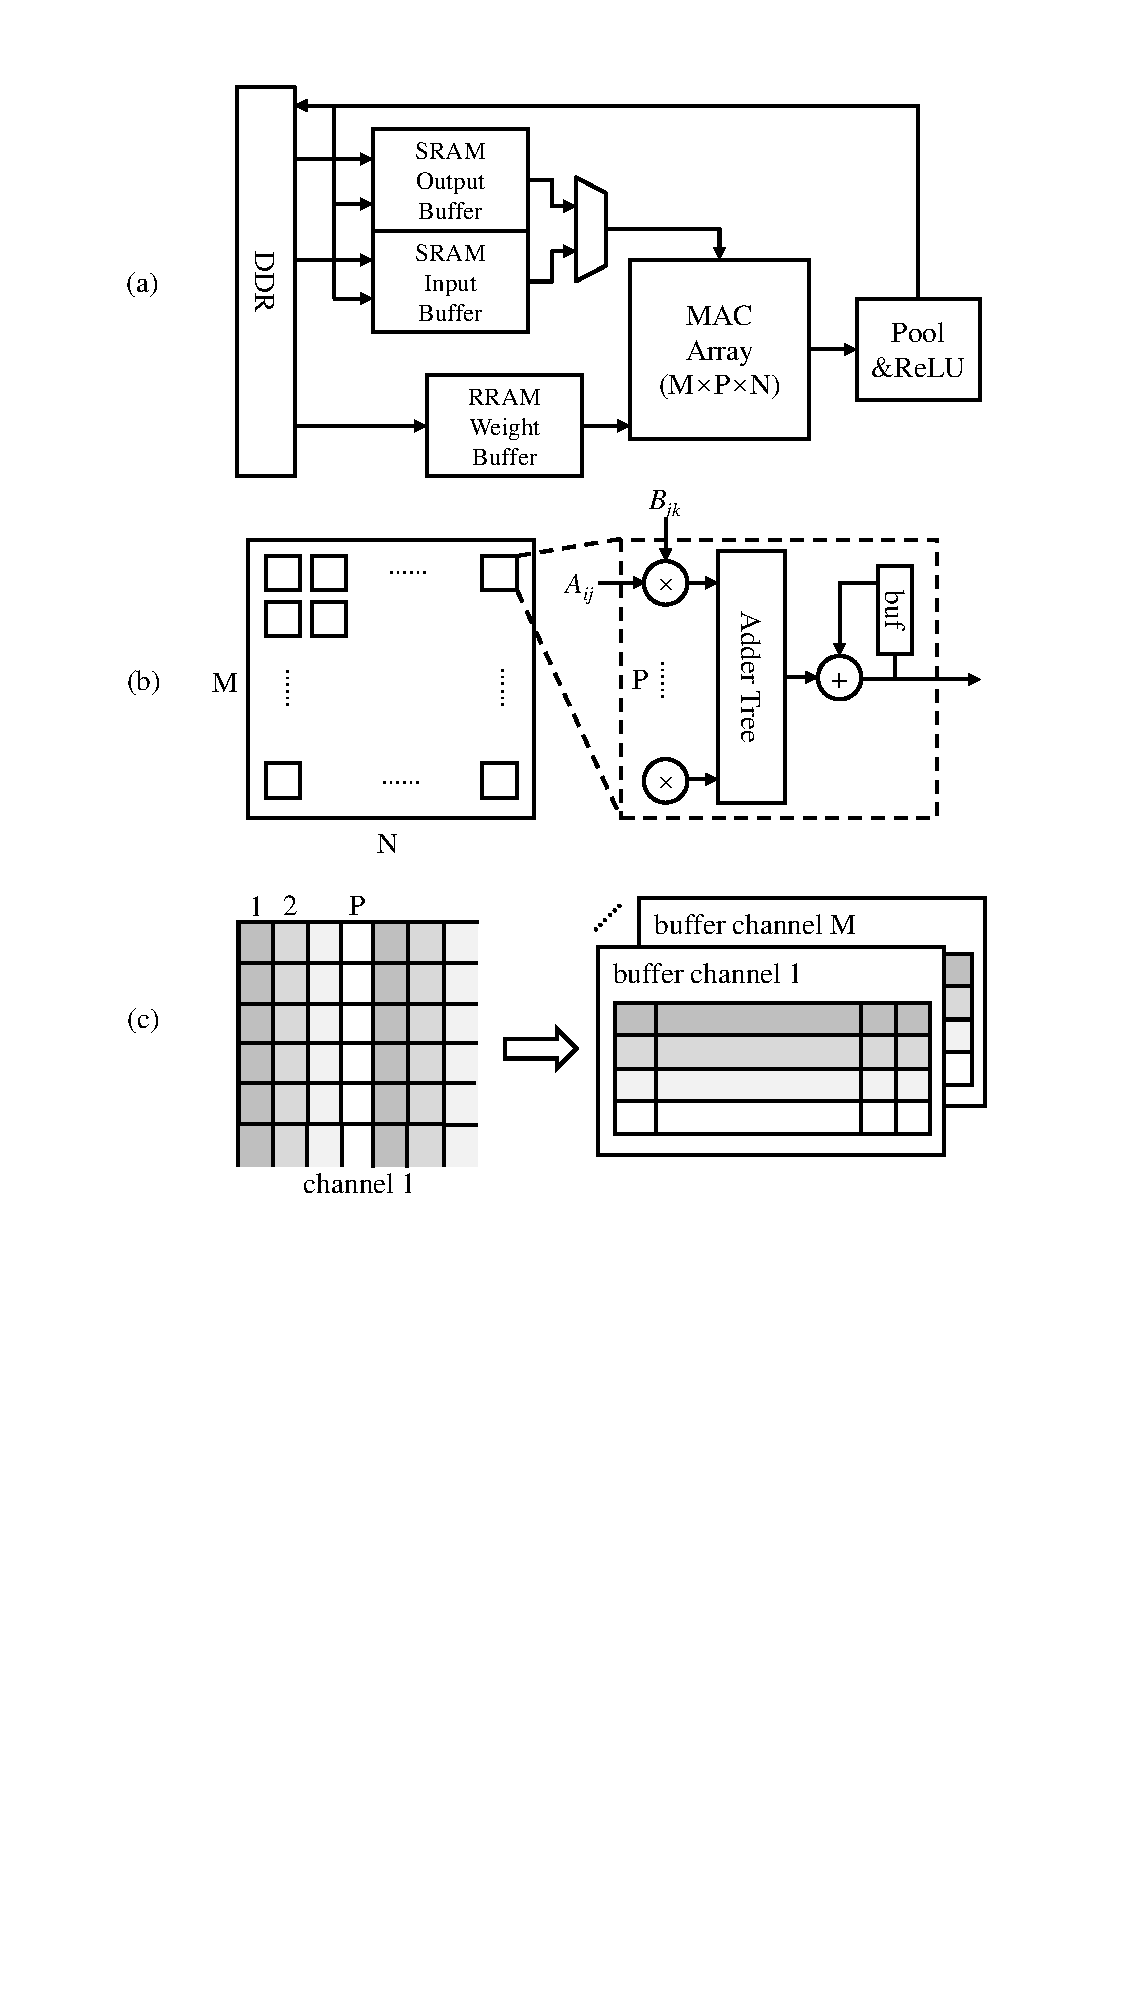
\includegraphics[width=1\columnwidth]{fig/arch.pdf}
      \caption{The CNN accelerator architecture. (a) The architecture mainly consists of a MAC array for computation and two levels of memory with on-chip buffers and external DDR. (b) Feature map buffer organization for sliding window data selection. (c) MAC array structure for an $A_{p\times m}\times B_{m\times n}$ matrix-matrix multiplication.}
      \vspace{-15pt}
      \label{fig:arch}
    \end{figure}
    
    The overall architecture is shown in Figure~\ref{fig:arch}(a). The system adopts DDR as external memory to support enough memory space. The on-chip memory consists of two buffers: input/output buffer and weight buffer. Input and output buffer stores feature maps during the process of a CNN. As the output of one layer serves as the input of the next, the input data of MAC array can be chosen from both of the buffers by a MUX unit. All the buffers works in a double-buffer way to cover the off-chip data transfer time with calculation time.
    
    We first show how the process of CNN is parallelized with this design. As introduced in Section II A, a CNN layer consists of 4 nested loops. In this case, we unroll the feature map pixel loop, input channel loop and output channel loop as a $A_{p\times m}\times B_{m\times n}$ matrix-matrix multiplication. Each row of matrix A denotes the p pixels read from a feature map and each $B_{ij}$ denotes a pixel in the convolution kernel corresponds to input channel $i$ and output $j$. Thus the convolution of $p$ pixels with $K\times K$ convolution kernels will be done with $\lceil M/m\rceil*K^2$ steps. 
    
    To support the above function, a window selection function is needed for each channel stored in input/output buffer. In this design, we adopt the data mapping format as shown in Figure~\ref{fig:arch}(b). The pixels of each channel are stored in $p$ independent RAMs so that a size-$p$ window at any position can be selected from the buffer within a single cycle. Weight buffer can be implemented with a normal simple dual port RAM.
    
    The structure of the computation core is shown in Figure~\ref{fig:arch}(c). The array consists of $p\times n$ PEs. Each of the PE implements a size-$m$ vector inner product in a pipelined manner. Each PE has an accumulator for its result. 
    
    \subsection{Energy Model}
    We only focuses on memory access energy, computation energy and background energy in this work. 
    
    For the memory access energy, we count the number of data read from or write to each buffer and multiplies them with a statistical energy cost generated from simulation tools. This highly relates to the schedule strategy because it decides how data is reused during the process of a CNN.
    
    For the computation energy, we calculate it by multiply the average energy cost of one operation, i.e. addition and multiplication, with the total number of operations in a network. So this part is fixed regardless of the schedule strategy or hardware design.
    
    For the background energy, we sum all the background power and multiplies it with the total processing time. The processing time of a network is given layer by layer, as the longer one between off-chip data transfer time and computation time.
    
    With the hardware design and the target network given, the computation energy cannot be optimized. Neither the background energy can be optimized if the system is not bounded by bandwidth. So we mainly focus on off-chip data transfer energy, which is decided by schedule strategy and the on-chip buffer energy for computation.
    
    \subsection{RRAM Buffer and Hardware Optimization}
    Consider the data access pattern, implement input/output buffers with RRAM is not practical. First, they require high write bandwidth to receive computation results from fast on-chip logic. Second, they require a high random access bandwidth, not sequential access bandwidth. Compared with input/output buffer, weight buffer only requires a high sequential access bandwidth. So in this work, we only consider the case where weight buffer is implemented with RRAM.
    
    As RRAM has high read/write dynamic, we should try to reuse the weight to reduce access to weight buffer. Here we use a small buffer rather than a register for the accumulation in PE as shown in Figure~\ref{fig:arch}(c). Each time a weight is read from weight buffer, we can utilize the buffer to store intermediate result for different output pixels before moving on to the next weight. With a buffer of size $d$, the time a weight will be read from weight buffer is expressed as equation~\ref{eqt:nw_read}
    
    \begin{equation}\label{eqt:nw_read}
      N_w = \lceil \lceil \frac{F_{out}.x * F_{out}.y}{p}\rceil \slash d \rceil
    \end{equation}
    
    Though this method reduce weight access to approximately $1/d$, more buffer energy is needed as $d$ increases. We search for the optimal point in our experiment.
    
    \section{Scheduling Strategy}
    In this section, we analyze schedule strategy, which decides the off-chip data transfer behavior during the process of a network. Three levels of schedule is considered: single layer, cross layer and network weight arrangement.
    
    \subsection{Single Layer Schedule Strategy}
    
    \begin{figure}[t]
      \centering
      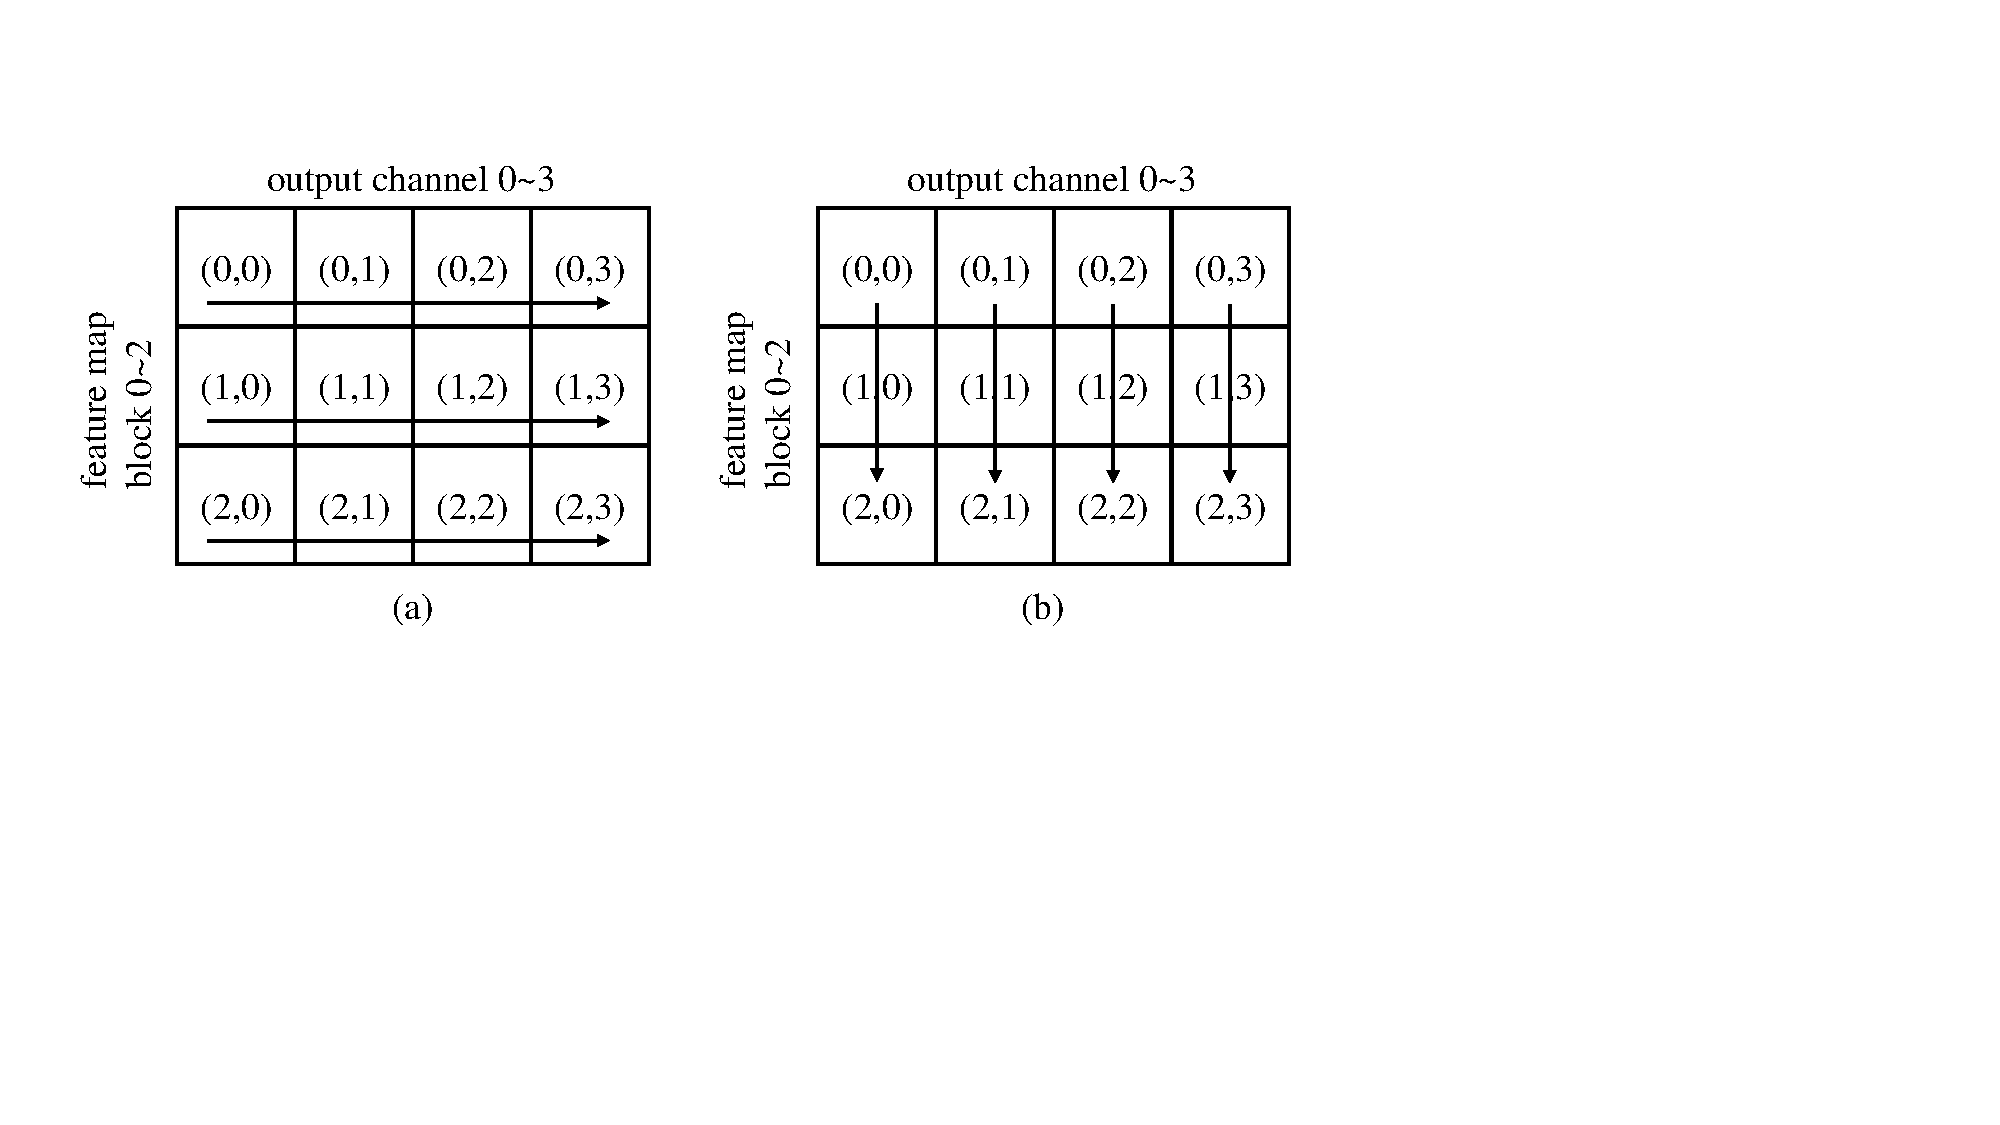
\includegraphics[width=1\columnwidth]{fig/single_layer.pdf}
      \caption{An example of how loop order affects data transfer behavior. Block $(i, j)$ denotes the computation for the $i^{th}$ feature map block on the $j^{th}$ channel. (a) Reuse feature map first and load each weight 3 times. (b) Reuse weight first and load each feature map 4 times.}
      \label{fig:single_layer}
    \end{figure}
    
    In the case where on-chip buffer size is smaller than the weight size and feature map size of a single layer, data needs to be loaded multiple times. An example is shown in Figure~\ref{fig:single_layer} where the weight buffer can hold only $1/4$ of the weight and input buffer can hold only $1/3$ of the feature maps. Choosing reuse weights or reuse feature map will cause difference on data transfer behavior and further affects the data transfer energy and data transfer time.
    
    \subsection{Cross Layer Schedule Strategy}
    \begin{figure}[t]
      \centering
      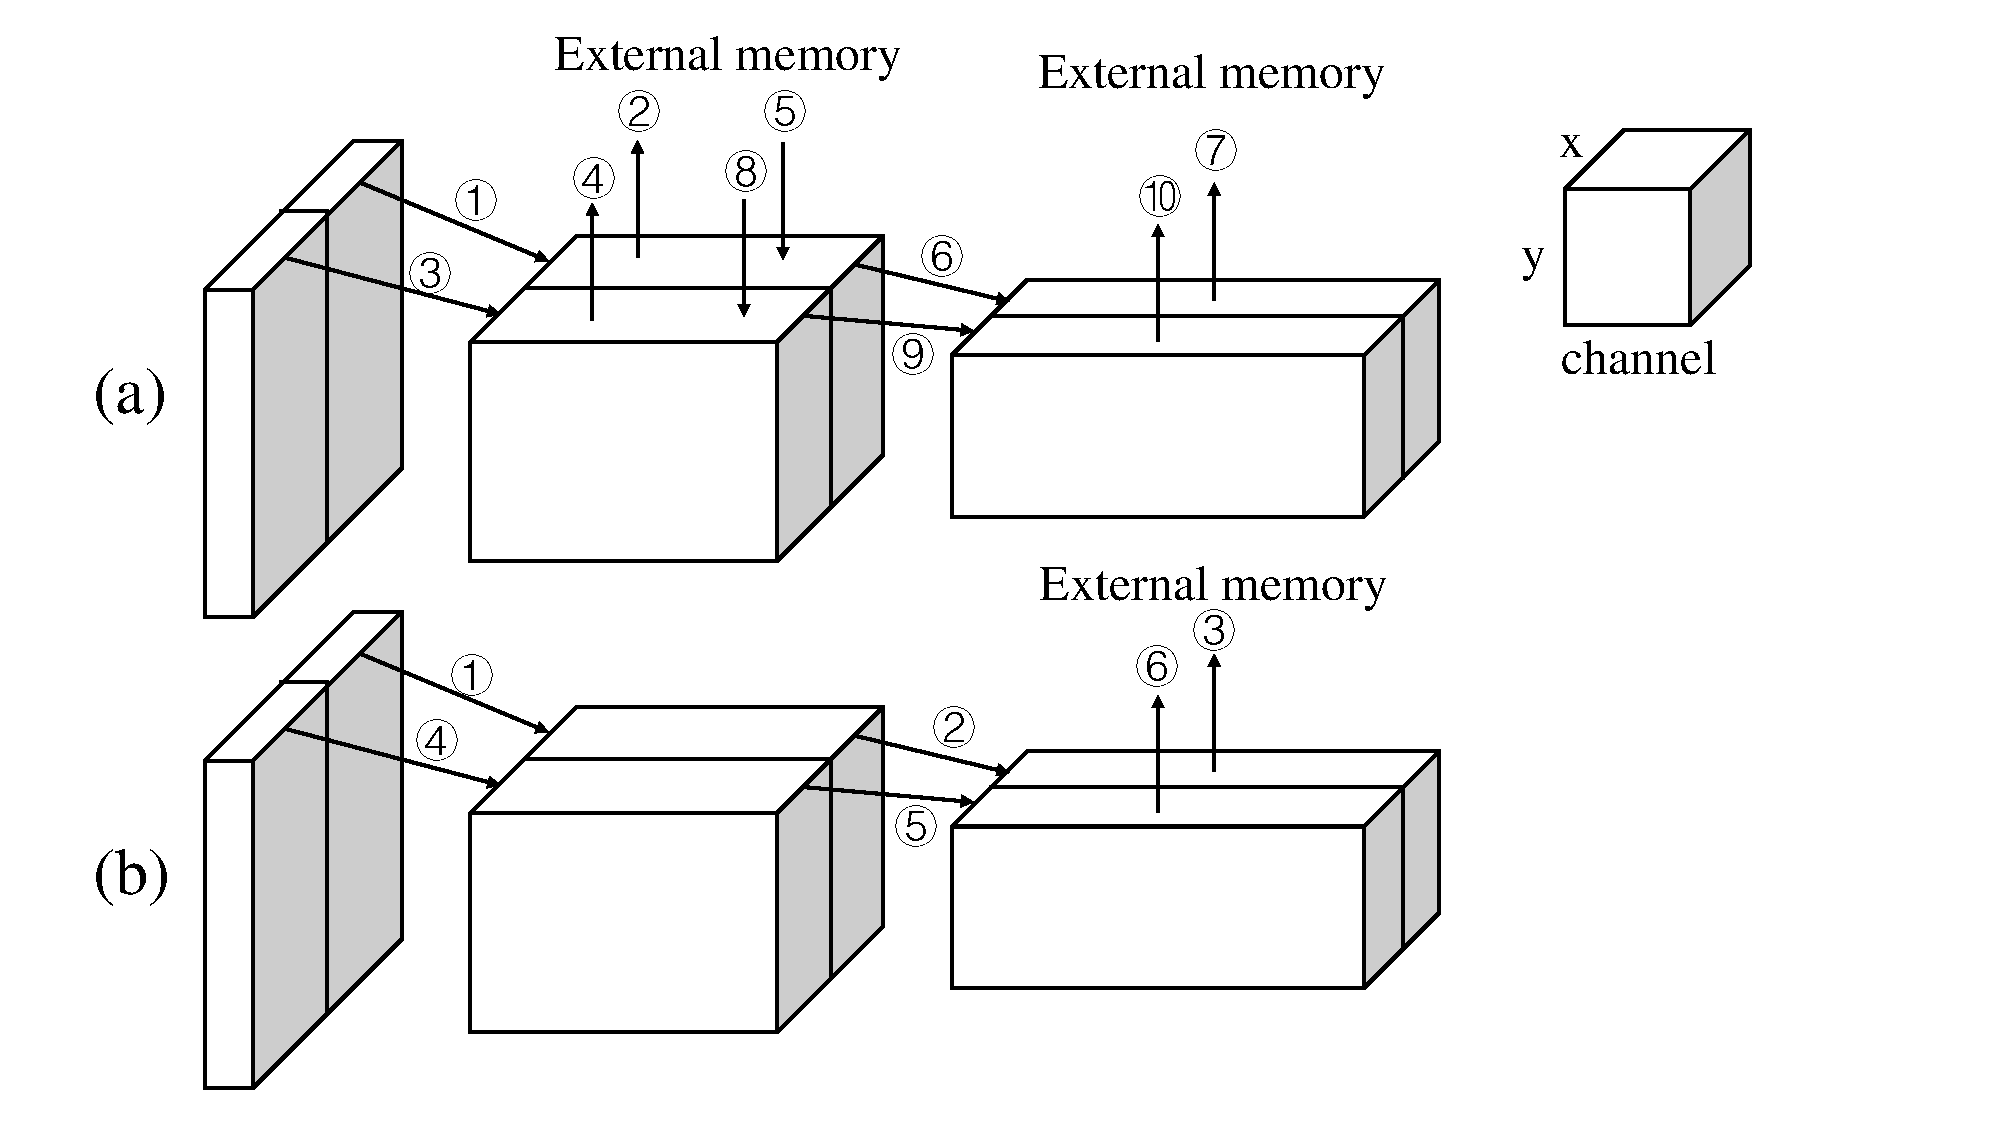
\includegraphics[width=1\columnwidth]{fig/cross_layer.pdf}
      \caption{An example of a cross layer schedule over 3 layers. (a) Single layer schedule. (b) Cross layer schedule.}
      \label{fig:cross_layer}
    \end{figure}
    
    As suggested by~\cite{alwani2016fused}, when the network is processed layer by layer, the result of one layer needs to be written back to external memory it is larger than the output buffer. But if the weight buffer is large enough to contain more than one layers' weight, these layers can be scheduled together to avoid writing the intermediate layers result to external memory. An example is shown in Figure~\ref{fig:cross_layer}, where the cross layer schedule avoids the second layer's feature map to be transferred to and from external memory. As we will implement weight buffer with RRAM, the size of weight buffer can be much larger and thus benefits from this strategy.
    
    \subsection{Network Weight Arrangement}
    An observation is that if the weight buffer is large enough to hold all the layer's weight on-chip, no weight will need to be read from external memory. With a slightly smaller buffer, we can still follow this idea by fix some of the layer's weights in on-chip buffer to reduce external memory access. So we need to find which layers' weight is to be fixed in the buffer as to minimize the total energy cost.
    
    The solution space of this problem is a depth-$(n+1)$ binary tree. $n$ denotes the number of CNV layers in the network. To avoid searching the whole $O(2^n)$ solution space, we prune the binary tree with the buffer size limitation. If the the weights on a path already exceeds the weight buffer size, we ignore the search of its subtree. The pseudo code of the optimization process is as follows:
    
    \begin{codebox}
    \Procname{\proc{SearchFixedWeight($layers$)}}
    \li Let $is\_fixed[1 .. \attrib{layers}{size}]$ be a boolean vector
    \li IterSearchFixedWeight($layers, 1, is\_fixed$)
    \li \Return $is\_fixed$
    \end{codebox}
    
    \begin{codebox}
    \Procname{\proc{IterSearchFixedWeight($layers, n, f$)}}
    \li \If $l > \attrib{layers}{size}$
    \li	\Do
         \Return OptEnergy($layers, f$)
      \End
    \li \If available buffer size $< \attrib{layers[n]}{weight\_size}$
    \li	\Do
         $f[n] = false$
    \li 	\Return IterSearchFixedWeight($layers, n+1, f$)
      \End
    \li $f1 = f$; $f1[n] = false$
    \li $f2 = f$; $f2[n] = true$
    \li $e1 =$ IterSearchFixedWeight($layers, n+1, f1$)
    \li $e2 =$ IterSearchFixedWeight($layers, n+1, f2$)
    \li \If $e1 < e2$
    \li	\Do
         $f = f1$
    \li 	\Return $e1$
    \li	\Else
    \li 	$f = f2$
    \li 	\Return $e2$
      \End
    \end{codebox}
    
    \section{Experiments}
    
    % Table generated by Excel2LaTeX from sheet 'ram config'
\begin{table*}[htbp]
  \centering
  \caption{Device parameters used for I/O buffer, weight buffer and DDR.}
    \begin{tabular}{|r|r|r|r|r|r|r|r|r|}
    \hline
          & bitwidth (B) & size (B) & Rd BW (GB/s) & Wr BW (GB/s) & Rd Ene (pJ) & Wr Ene(pJ) & Leakage (mW) & Area (um\^2)\\
    \hline
    \multicolumn{1}{|c|}{} & 32    & 128K  & 15.169  & 1.556  & 67.690  & 195.286  & 0.04000  & 21224 \\
\cline{2-9}    \multicolumn{1}{|c|}{22nm} & 32    & 256K  & 11.693  & 1.534  & 75.071  & 217.468  & 0.04104  & 26707 \\
\cline{2-9}    \multicolumn{1}{|c|}{LSTP} & 32    & 512K  & 8.005  & 1.490  & 88.483  & 260.073  & 0.04314  & 37308\\
\cline{2-9}    \multicolumn{1}{|c|}{RRAM} & 32    & 1M    & 11.056  & 1.534  & 133.189  & 268.319  & 0.05282  & 61090 \\
\cline{2-9}    \multicolumn{1}{|c|}{} & 32    & 2M    & 10.306  & 1.534  & 231.750  & 357.190  & 0.07806  & 107007 \\
    \hline
    \multicolumn{1}{|c|}{} & 8     & 16K   & 9.145  & 5.147  & 3.057  & 0.556  & 0.00134  & 10031 \\
\cline{2-9}    \multicolumn{1}{|c|}{22nm} & 8     & 32K   & 8.609  & 4.973  & 6.432  & 1.315  & 0.00270  & 20048 \\
\cline{2-9}    \multicolumn{1}{|c|}{LSTP} & 8     & 64K   & 16.831  & 11.763  & 6.780  & 3.777  & 0.00600  & 42803 \\
\cline{2-9}    \multicolumn{1}{|c|}{SRAM} & 8     & 128K  & 10.977  & 10.451  & 7.931  & 2.792  & 0.01153  & 82032 \\
\cline{2-9}    \multicolumn{1}{|c|}{} & 8     & 256K  & 10.977  & 10.451  & 11.562  & 6.424  & 0.02306  & 164065 \\
    \hline
    \multicolumn{1}{|c|}{DDR4} & 4    & 128M  & \multicolumn{2}{c|}{3.2} & 80.300  & 82.719  & 52.80000  & N/A \\
    \hline
    \end{tabular}%
  \label{tab:device}%
\end{table*}%
    
    Experiments are carried out on the architecture introduced in Section III, with the scheduling strategy in section IV applied. Design space exploration is also done to optimize the energy cost of a state-of-the-art network.
    
    \subsection{Experiment setup}
    The MAC array in the architecture is configured as an $8\times8\times8$ array running at 1GHz. This offers a peak performance of 1TOP/s. 8bit multiplication and 32bit accumulation is adopted in this model. Multiplication and addition energy is scaled down from the data in~\cite{mac_energy} to 22nm technology. 
    
    The above configuration requires the read bandwidth of input/output buffer and weight buffer to be at least 64GB/s. We implement each buffer with 8 banks and each of them should offer 8GB/s read bandwidth. On-chip memory parameters are generated from NVSim~\cite{dong2014nvsim} with different memory size configuration. To achieve enough bandwidth, RRAM buffer bit width is configured as 256bit. 
    
    The external memory parameter is generated from MICRON DDR4 power calculator~\cite{powercalc}. The generated dynamic I/O power is further converted to energy per read or write byte. In our experiment, we use 2 DDR chips as external memory because the bandwidth can support the configured MAC array with proposed schedule strategy and the size is enough. In order to reduce background power overhead, we use the least number of chips. All the detailed data and configuration is shown in Table~\ref{tab:device}. 
    
    The buffer in the accumulator is also considered in our experiments. 4 types of buffer is chosen for design space exploration. Corresponding parameters are generated by NVSim and are shown in Table~\ref{tab:small_buf}
    
    \begin{table}[htbp]
  \centering
  \caption{32-bit accumulation buffer parameters.}
    \begin{tabular}{|r|r|r|r|r|}
    \hline
    depth & 16    & 32    & 64    & 128 \\
    \hline
    energy per read (pJ) & 0.045 & 0.056 & 0.107 & 0.12 \\
    \hline
    energy per write (pJ) & 0.022 & 0.031 & 0.083 & 0.094 \\
    \hline
    \end{tabular}%
  \label{tab:small_buf}%
\end{table}%
    
    \subsection{DDR Access energy optimization}
    
    \begin{figure}[t]
      \centering
      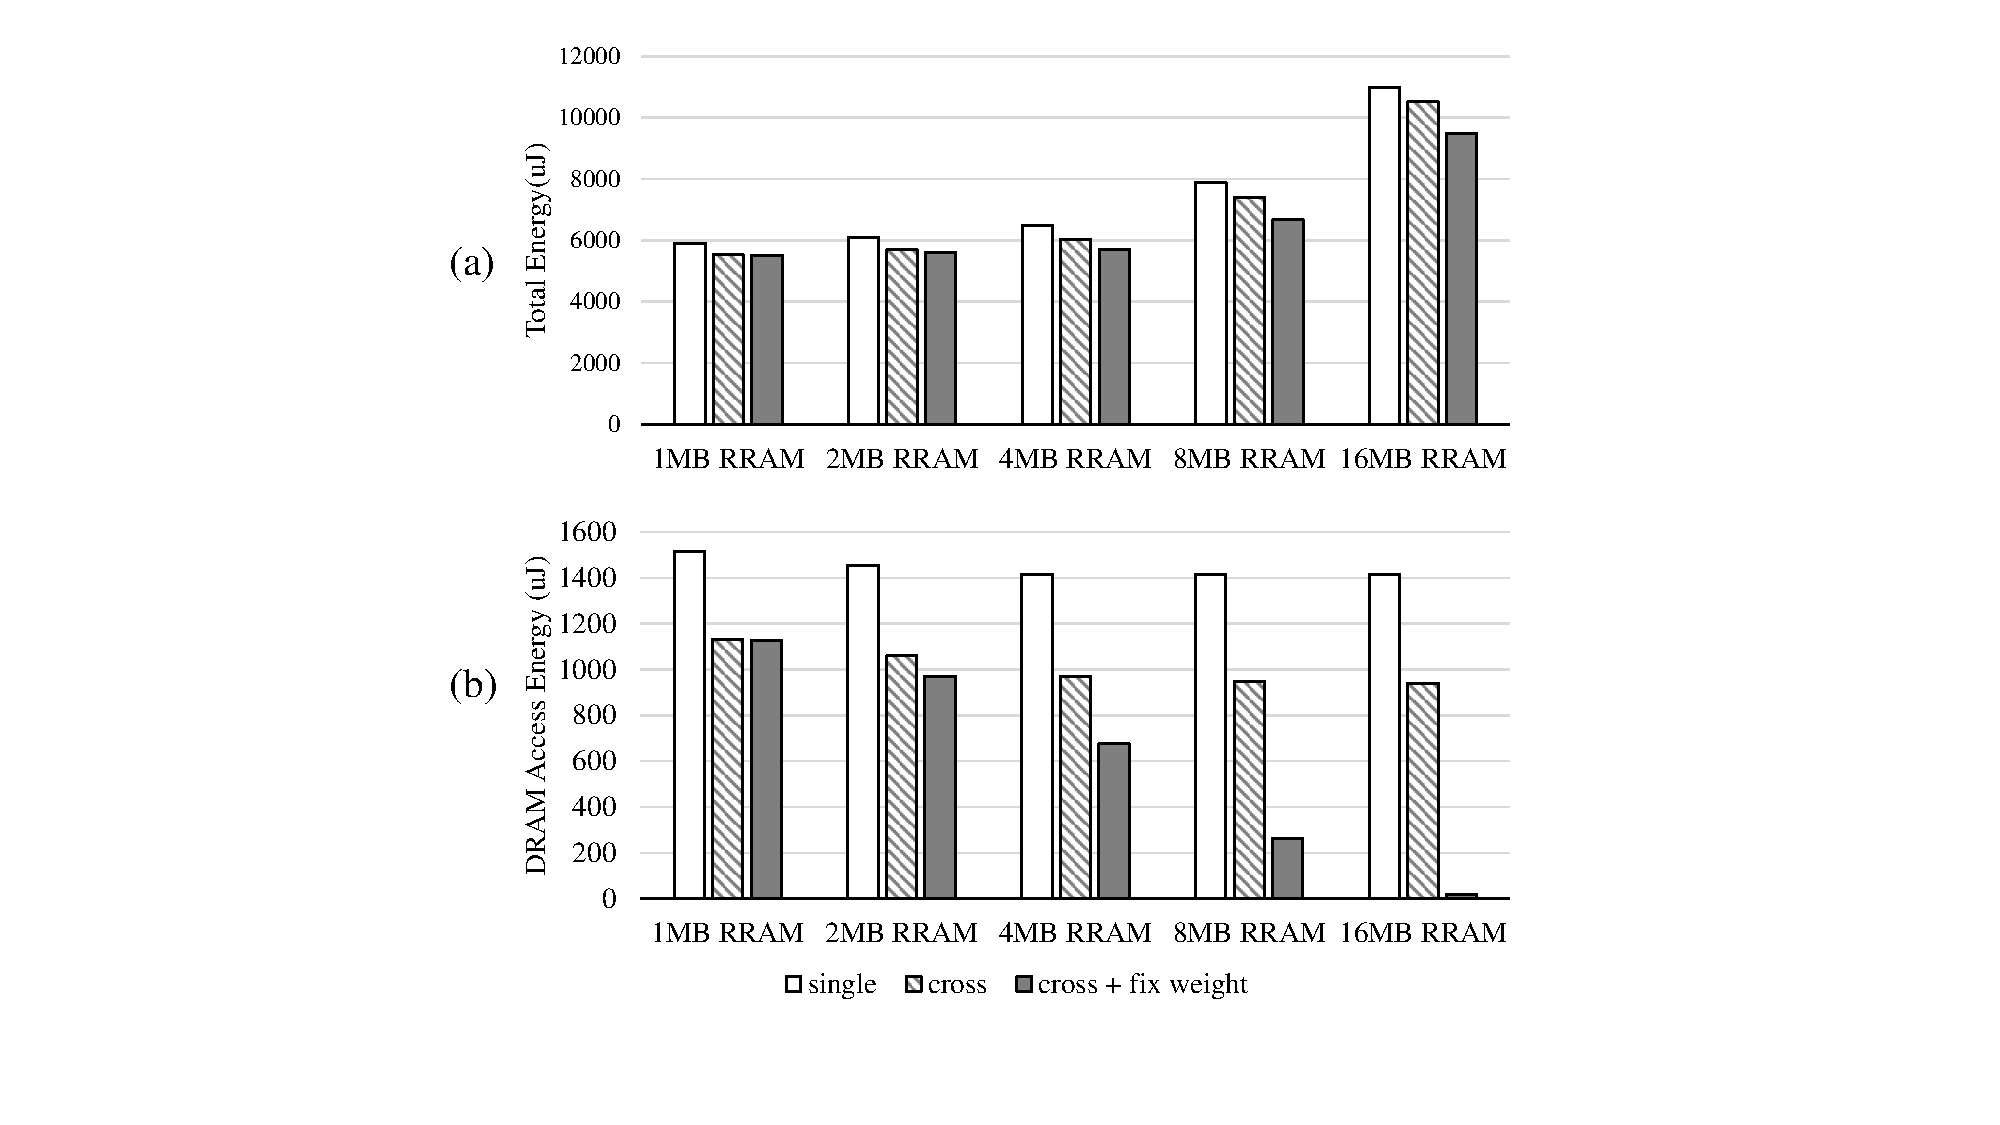
\includegraphics[width=1\columnwidth]{fig/opt_res.pdf}
      \caption{System energy with different level of schedule optimization. (a) Total system energy. (b)DRAM access energy.}
      \label{fig:exp_strategy}
    \end{figure}
    
    DDR access behavior is totally decided by schedule strategy. Here we use the convolution layers of VGG-11 to test the effectiveness of the schedule strategy optimization. Figure~\ref{fig:exp_strategy} shows the experimental results. Input/output buffer is 128KB SRAM and weight buffer varies from 1MB to 16MB RRAM in this experiment. Three levels of optimization is compared: only single layer schedule, cross layer schedule, cross layer schedule and consider fixing weight in buffer. When the weight buffer is small, the main energy saving comes from the cross layer schedule. When the buffer gets larger, fixing weight becomes more important. Up to $20\%$ energy saving can be achieved by the our schedule strategy optimization. From Figure~\ref{fig:exp_strategy}(b), we see that strategy optimization reduces the DDR access energy by $25\%\sim 98\%$ under different memory configurations.
    
    \subsection{On-chip buffer energy optimization}
    From Figure~\ref{fig:exp_strategy}(a), we see that using a larger buffer is not better. This is caused by the increasing buffer I/O energy and leakage power. An example of energy breakdown is shown in Table~\ref{tab:ene_comp}. Both of the design adopts 1MB SRAM I/O buffer. The SRAM weight buffer is 128KB and the RRAM weight buffer is 1MB. Though the RRAM design has less DDR access energy because of a larger weight buffer, the weight buffer read energy is much higher. This shows the necessity of using buffer, rather than a single register, for accumulation. 
    
    \begin{table}[htbp]
  \centering
  \caption{Example energy breakdown for a pair of SRAM and RRAM design}
    \begin{tabular}{|r|R{1cm}|r|R{1cm}|r|}
    \hline
          & \multicolumn{2}{c|}{RRAM weight buffer} & \multicolumn{2}{c|}{SRAM weight buffer} \\
    \hline
    read iobuf & 0.29  & 0.01\% & 0.29  & 0.01\% \\
    \hline
    read weight & 2119  & 40.50\% & 383   & 10.85\% \\
    \hline
    read ddr & 841   & 16.10\% & 929   & 26.34\% \\
    \hline
    write iobuf & 1.04  & 0.02\% & 1.04  & 0.03\% \\
    \hline
    write weight & 50.4  & 0.96\% & 0.64  & 0.02\% \\
    \hline
    write ddr & 2.08  & 0.04\% & 2.08  & 0.06\% \\
    \hline
    standby & 1691  & 32.33\% & 1686  & 47.79\% \\
    \hline
    calculate & 526   & 10.05\% & 526   & 14.90\% \\
    \hline
    Total & 5230  &       & 3527  &\\
    \hline
    \end{tabular}%
  \label{tab:ene_comp}%
\end{table}%
    
    We still use the VGG-11 convolution layers to search for an optimal accumulator buffer depth. For each depth choice, we search the optimal buffer size configuration with all the schedule strategy optimization applied. The results are shown in Figure~\ref{fig:exp_buf_depth}. As can be seen from the figure, both methods benefits from the accumulation buffer, but the RRAM design benefits more. With the accumulation buffer, the total on-chip buffer energy cost can be reduced by $86\%$. Combining schedule optimization and accumulation buffer design, we can finally achieve $18\%$ energy reduction by introducing RRAM into on-chip buffer design.
    
    \begin{figure}[t]
      \centering
      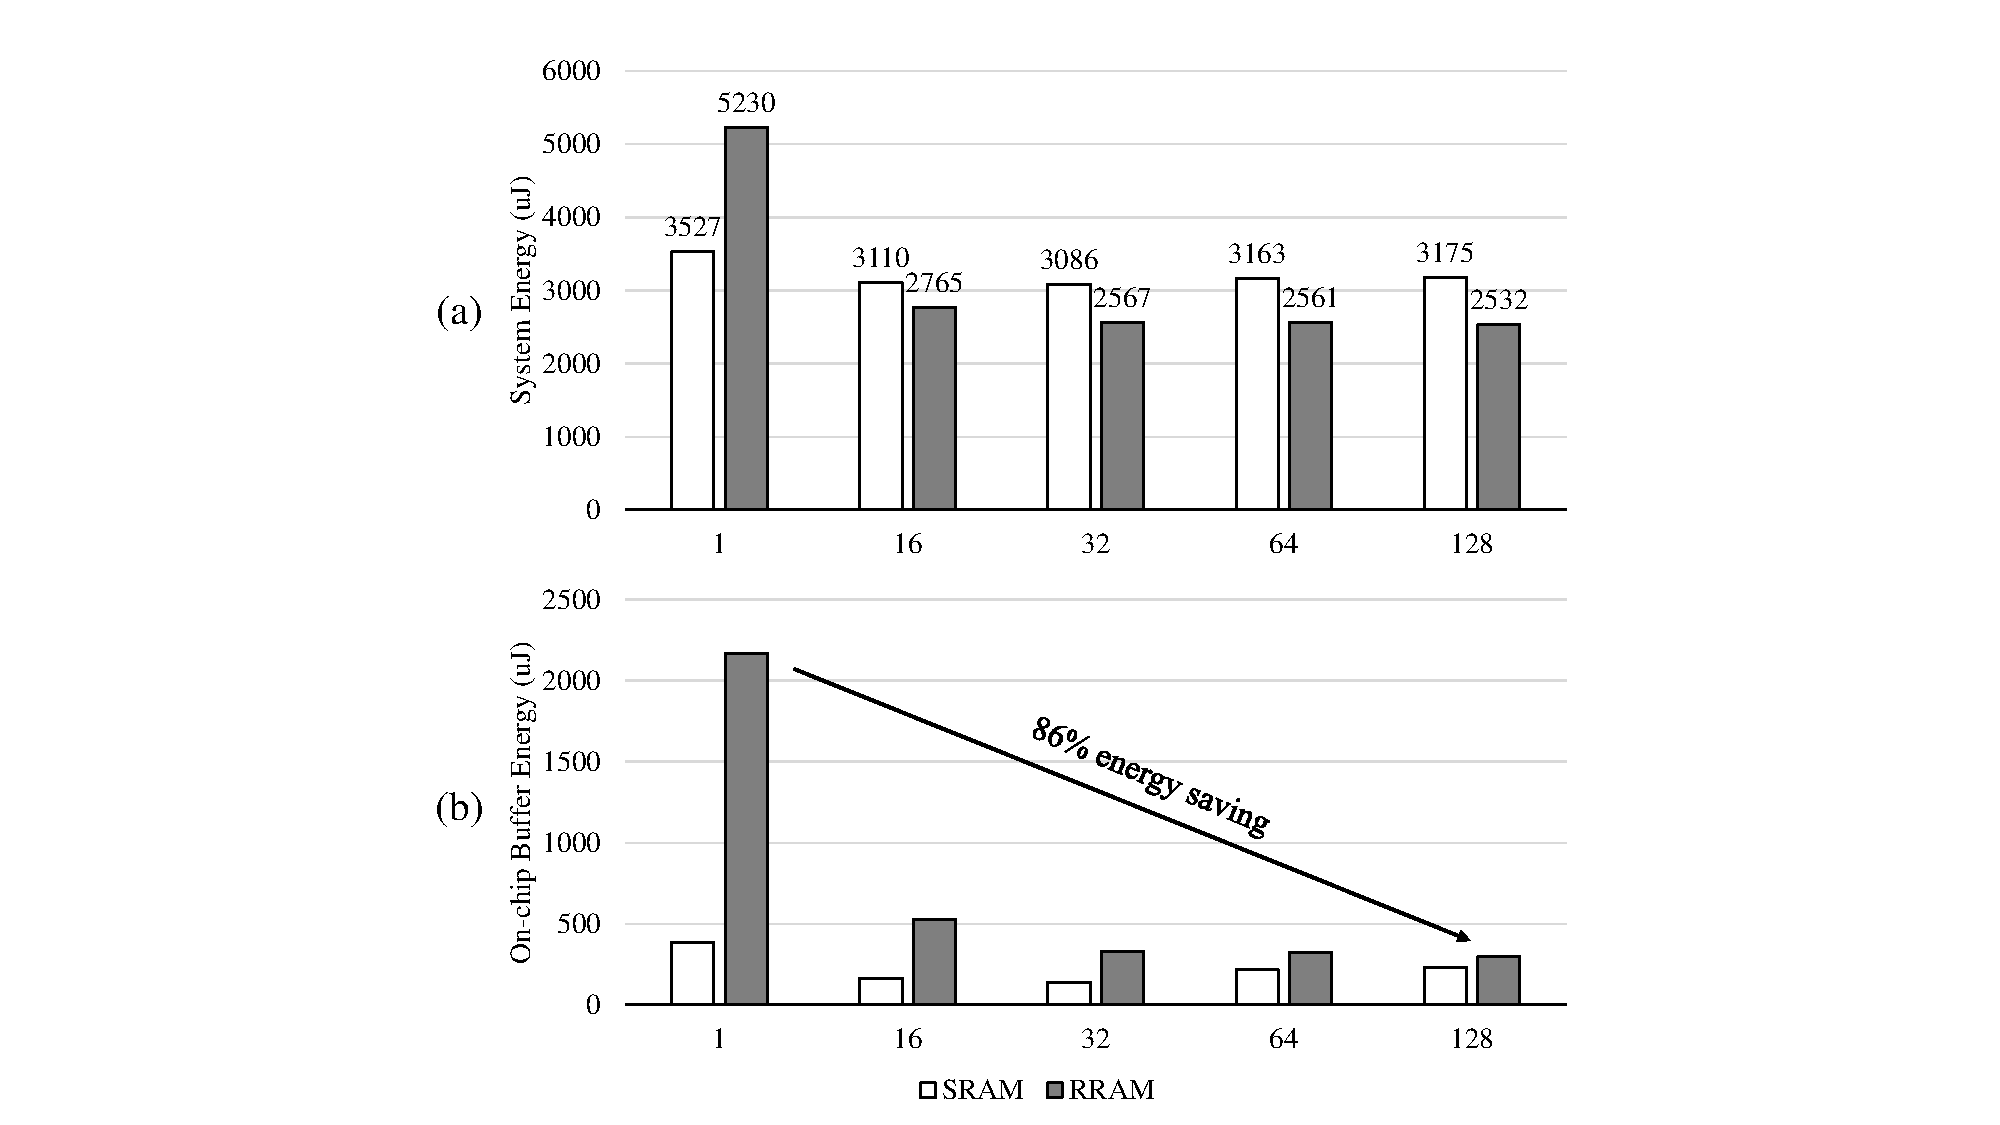
\includegraphics[width=1\columnwidth]{fig/buf_size.pdf}
      \caption{System energy with different accumulation buffer size. (a) System energy cost. (b) On-chip buffer energy cost.}
      \label{fig:exp_buf_depth}
    \end{figure}
    
    \section{Conclusion}
    In this paper, we try to introduce RRAM into CNN accelerator on-chip buffer design. The accumulation buffer is introduced to relief the I/O energy overhead brought by RRAM. A set of schedule strategy optimizations is proposed to fully utilize the high storage density of RRAM. Experimental results show that by combining the hardware and software optimization and do design space exploration, $25\%\sim 98\%$ DRAM access energy and $86\%$ on-chip buffer energy can be saved. RRAM based design achieves 18$\%$ less system energy compared with an SRAM based design. Future work should focus on the rest part of the energy cost like the standby energy and the computation energy.
    
    \small
    \bibliographystyle{IEEEtran}
    \bibliography{ref}
    
    
    \end{document}
    